\section{Planificación, Fases e iteraciones}\label{cap:planificacionExtensa}

\subsection{Planificación inicial}

Este proyecto consta de tres grandes fases, cuya planificación general se puede observar en el siguiente Diagrama de Gantt \cite{diagramaGantt} (Figura \ref{fig:DiagramaGanttCompleto}): una primera fase de análisis, una segunda fase de desarrollo iterativo e incremental, organizada en cinco iteraciones, y una tercera y última fase de documentación y entrega.

\begin{figure}[H]
    \centering
    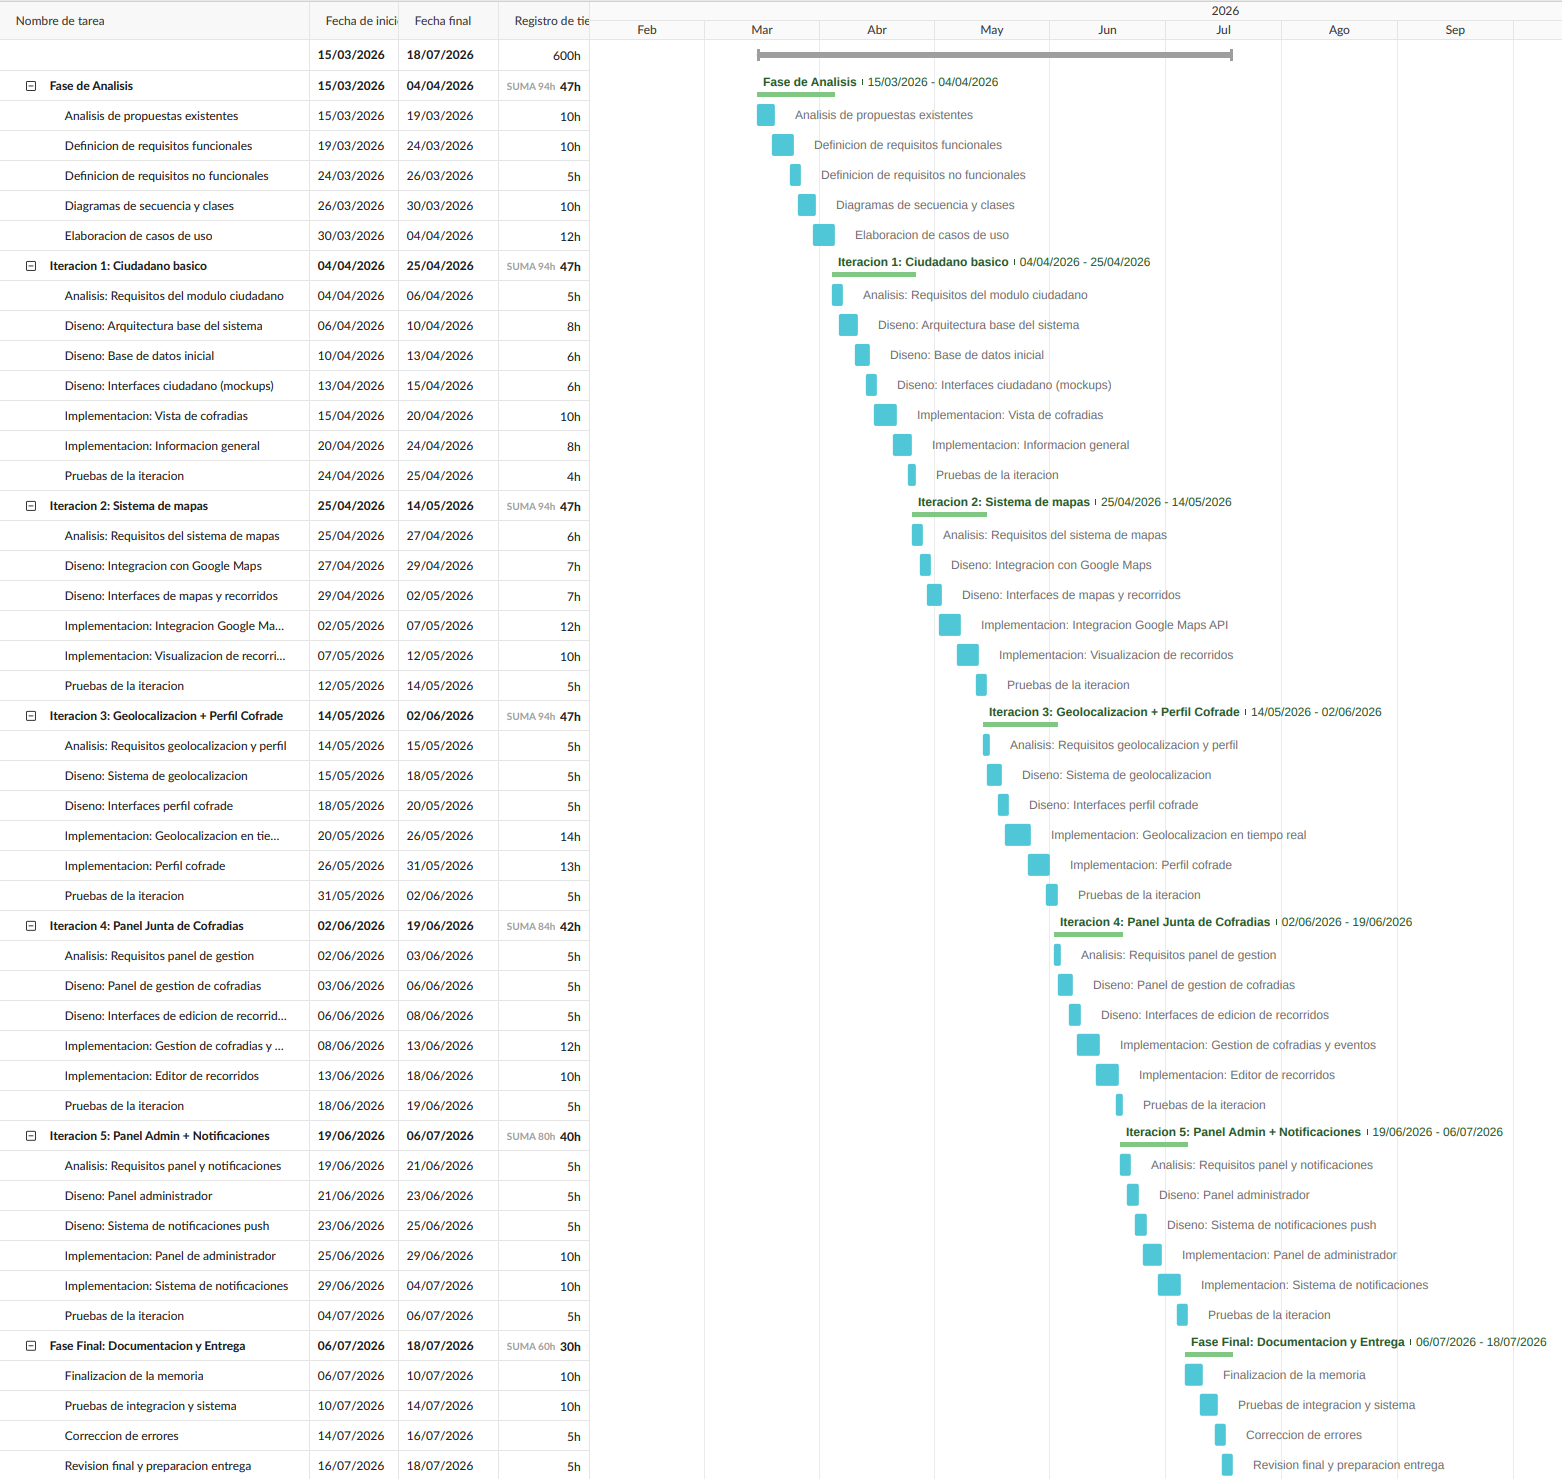
\includegraphics[width=1\textwidth]{imagenes/DiagramaGantBig.png}
    \caption{Diagrama de Gantt general completo del proyecto}
    \label{fig:DiagramaGanttCompleto}
\end{figure}

\subsection{Fase de análisis}

Esta primera fase se centra en el análisis de las aplicaciones relacionadas con la Semana Santa existentes, la identificación de sus carencias y áreas de mejora, y en la definición extendida de los requisitos funcionales y no funcionales \cite{ieee29148} del sistema, además de la elaboración de los casos de uso \cite{uml} y los distintos diagramas que servirán como base para la realización del desarrollo de la aplicación.

Esta fase comienza con el análisis de las propuestas existentes en el mercado, identificando las características principales de aplicaciones como \textit{El Penitente} \cite{elpenitente}, \textit{Valladolid Cofrade} \cite{valladolidCofrade} o \textit{sSantaZgz} \cite{sSantaZgz}.

Seguido de este análisis se realiza la definición de los requisitos funcionales, los cuales describen las funcionalidades concretas que el sistema debe ofrecer, y los requisitos no funcionales, que definen las condiciones de calidad, rendimiento y seguridad que debe cumplir \cite{ieee29148}, teniendo en cuenta los cuatro perfiles de usuario: ciudadano, cofrade, Junta de Cofradías y administrador. También se elaboran los diagramas de secuencia y el modelo de dominio, así como los casos de uso \cite{uml}, representaciones estandarizadas de las interacciones entre los usuarios y el sistema, que servirán para el desarrollo posterior.

\subsection{Fase de iteraciones}

Esta segunda fase está centrada en el diseño e implementación de la aplicación de forma iterativa e incremental \cite{larman2004}. Aunque el marco general del proyecto sigue el modelo en cascada --en el sentido de que el análisis es seguido del diseño y tras este la implementación--, en esta fase se aplica un ciclo interno de análisis, diseño, implementación y pruebas en cada iteración, lo que permite ir incorporando las funcionalidades de forma progresiva y verificando su correcto funcionamiento antes de darla por finalizada y avanzar a la siguiente. El desglose detallado de tareas y horas de cada iteración puede consultarse en el Diagrama de Gantt (Figura~\ref{fig:DiagramaGanttCompleto}).

Estas iteraciones abarcan desde las funcionalidades básicas del ciudadano hasta las más complejas, como la geolocalización en tiempo real, es decir, la capacidad de conocer y actualizar la posición geográfica de una procesión de forma continua haciendo uso de la tecnología GPS\footnote{GPS (Global Positioning System): sistema de navegación por satélite que permite determinar la posición geográfica de un dispositivo en cualquier punto del planeta.} del móvil, o el sistema de notificaciones (mensajes enviados desde el servidor a los dispositivos de los usuarios sin que estos tengan que abrir la aplicación activamente).

\subsubsection{Iteración 1: Módulo ciudadano básico}

Esta primera iteración tiene como objetivo establecer la arquitectura base del sistema y desarrollar las funcionalidades fundamentales del perfil de ciudadano, entre las que se incluyen la visualización de la información general de la Semana Santa, el listado de organizaciones y la consulta de eventos.

\subsubsection{Iteración 2: Sistema de mapas}

Esta segunda iteración se centra principalmente en la implementación del sistema de mapas, que permitirá visualizar los distintos recorridos de las procesiones.

\subsubsection{Iteración 3: Geolocalización y perfil cofrade}

Esta tercera iteración se centra en la implementación completa del sistema de geolocalización en tiempo real, de forma que se pueda conocer y actualizar de manera continua la posición de las procesiones durante su recorrido. Además, se desarrolla el perfil de cofrade con sus correspondientes funcionalidades, incluyendo la posibilidad de compartir la ubicación durante las procesiones.

\subsubsection{Iteración 4: Panel de la Junta de Cofradías}

Esta cuarta iteración corresponde al desarrollo del panel de gestión para las Juntas de Cofradías, permitiendo administrar la información de la Semana Santa, incluyendo eventos, recorridos, imágenes y participantes. El acceso a este panel está restringido mediante un mecanismo de control de acceso \cite{owasp}, que permite diferenciar los permisos y limitaciones de los distintos roles del sistema.

\subsubsection{Iteración 5: Panel de administrador y notificaciones}

Esta quinta y última iteración se centra en la implementación del panel de administrador global del sistema, así como del sistema de notificaciones, que permitirá a la Junta de Cofradías comunicar a los usuarios cambios o incidencias en las procesiones de forma inmediata, sin necesidad de que estos tengan la aplicación abierta.

\subsection{Fase final: documentación y entrega}

En esta última fase se realizan las pruebas de integración del sistema completo, la corrección de errores detectados, la finalización de la memoria del proyecto y la preparación de la entrega final.
